\chapter{Polly}
Polly\footnote{The name \enquote{Polly} is combination of \enquote{Polyhedral} and \enquote{\llvm}. \cite{PollyGrosser}} is one of the numerous subprojects of \llvm and provides ways for automatic optimizations based on the polyhedral model operating on \llvmir.

\section{Geschichte}
Polly was first described in the publication \cite{PollyGrosser}. TODO: More information?

\section{The pipeline of Polly}
The optimizations implemented by Polly can be used by flags of the \opt when loading the library of Polly (\autoref{subsec:optimizer}).
\begin{figure}[h]
    \caption{Die Pipeline von Polly \cite{PollyPresentation}}
    \centering
    \begin{tikzpicture}
        \coordinate(clang);
        \node(opt)[llvmIrNode, right=of clang]{\ac{LLVM} Optimizer};
        \node(polly)[llvmIrNode, below=of opt]{\ac{LLVM} Polly};
        \coordinate[right=of opt](generator);
        \path[llvmIrPath] (clang) to (opt);
        \path[llvmIrPath, bend right] (opt.south west) to node[auto, swap]{SCoP Detection} (polly);
        \path[llvmIrPath, bend right] (polly) to node[auto, swap]{Code Generation} (opt.south east);
        \path[llvmIrPath] (opt) to (generator);
        \path[llvmIrPath] (polly) edge[loop below] ();
    \end{tikzpicture}
\end{figure}\\
There are two essential terms for understanding Polly. On the one hand it is \enquote{region} on the other hand it is \enquote{\scop}.
\subsection{Definition region}
In \cite[chapter 9.7.1, p.~672]{Drachenbuch} a region is defined as:
\begin{comment}
    Seite 672, Chapter 9. Machine-independent optimizations, 9.7.1 Regions
\end{comment}
\begin{quote}
    Formally, a region of a flow graph is a collection of nodes N and edges E such that:
    \begin{enumerate}
        \item There is a header h in N that dominates all the nodes in N.
        \item If some node m can reach a node n in N without going through h, then m is also in N.
        \item E is the set of all the control flow edges between nodes \(n_1\) and \(n_2\) in N, except (possibly) for some that enter h.
    \end{enumerate}
\end{quote}
In \autoref{fig:exampleRegion} some sourcecode and its corresponding regions are shown.
\begin{figure}
    \caption{A simple example of regions}
    \label{fig:exampleRegion}
    \begin{minipage}{.7\textwidth}
        \lstinputlisting[language=c++]{cpp/matmul.cpp}
    \end{minipage}
    \begin{minipage}{.2\textwidth}
        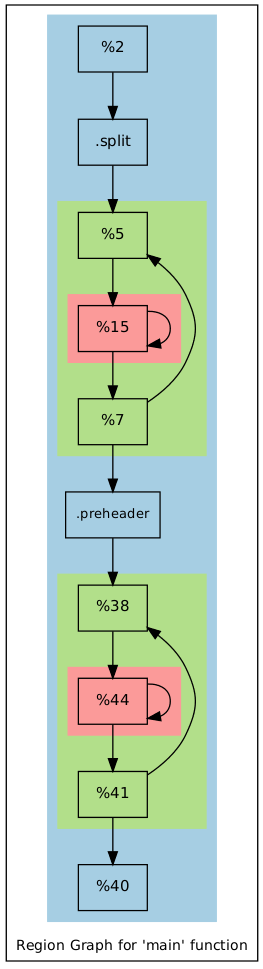
\includegraphics[height=12cm]{gfx/matmulRegions.png}
    \end{minipage}
\end{figure}
For visualizing the regions of this program a dot file was generated executing the following steps/commands:
\begin{enumerate}
    \item Translate the C++ sourcecode into \llvmir (\autoref{lst:matmulll})\\
        \texttt{clang -S -std=c++14 -O3 -emit-llvm matmul.cpp -o matmul.ll}
    \item Prepare the \llvmir for Polly (\autoref{lst:matmulpreoptll})\\
        \texttt{opt -load LLVMPolly.so -S -polly-canonicalize matmul.ll > matmul.preopt.ll}
    \item Generate a dot file\\
        \texttt{opt -load LLVMPolly.so -view-regions-only matmul.preopt.ll}
\end{enumerate}
\subsection{Definition SCoP}
